\documentclass[a4paper, amsfonts, amssymb, amsmath, reprint, showkeys, nofootinbib, twoside]{revtex4-1}
\usepackage[english]{babel}
\usepackage[utf8]{inputenc}
\usepackage[colorinlistoftodos, color=green!40, prependcaption]{todonotes}
\usepackage[pdftex, pdftitle={Article}, pdfauthor={Author}]{hyperref}
\usepackage{amsthm}
\usepackage{mathtools}
\usepackage{physics}
\usepackage{xcolor}
\usepackage{caption}
\usepackage{hyperref}
%\hypersetup{colorlinks=true, linkcolor=blue, urlcolor = blue}
\usepackage{amsmath}
\usepackage{amssymb}
\usepackage{graphicx}
\graphicspath{Images}
\usepackage[left=23mm,right=13mm,top=35mm,columnsep=15pt]{geometry} 
\usepackage{adjustbox}
\usepackage{placeins}
\usepackage[T1]{fontenc}
\usepackage{float}
%\usepackage{longtable}
\usepackage{csquotes}
\usepackage{refstyle}
\usepackage{lipsum}

\begin{document}

\title{Determination of excitation energy of Ne Atoms}
\author{Swaroop Ramakant Avarsekar}
\email{swaroop.avarsekar@niser.ac.in}
\affiliation{School of Physical Sciences, National Institute of Science Education and Research, HBNI, Jatni -752050, India}
\date{\today}

	
\begin{abstract}
Neon atoms are excited by accelerating the electrons from the cathode and resulting inelastic collision. The electrons in the atom absorb the energy and get excited to higher energy state. The most probable excitation for Neon atoms takes place from ground states to ten 3p states, which is 18.4 eV and 19.0 eV from the ground state. The de-excitation of the 3p states to the ground state with emission of a photon is only possible via the 3s states, resulting in emission of visible light. Three luminescence layers are visible in the neon tube indicating the excitation. Experimentally, we aim to determine this excitation energy. We obtained first excitation energy Ne as 19.438 eV which is close to the this range.
\end{abstract}
	
\keywords{Thermionic emission, Excitation, Quantised}
	
\maketitle

\section{Introduction}
In 1913, Niels Bohr proposed his atomic model for hydrogen and hydrogenic atoms predicting electron are occupied only specific energy levels in the atom. In 1914, James Franck and Gustav Hertz reported quantised energy loss for electrons passing through mercury vapour, and a corresponding emission at the ultraviolet line of mercury, with wavelength corresponding to $\lambda=253.6 nm$. Electrons below certain threshold limit fail to give any electromagnetic radiation. This observation confirmed Bohr's model of hydrogen atom, hence led to development of quantum theory.

\section{Theory}\label{theo}
The ground state electronic configuration of Neon is $1s^{2}2s^{2}2p^{6}$. Neon atoms are filled in the Franc-Hertz tube. Thorium activated tungsten filament in cathode is used to emit the electrons by thermionic emission, by heating the filament by applying voltage. These filaments have long lifetimes and resistance to ion bombardment at high voltages, since thorium continuously diffuses to surface renewing the layer. 
Neon atoms are excited by accelerating the electrons from the cathode and resulting inelastic collision. The electrons in the atom absorb the energy and get excited to higher energy state. The most probable excitation for Neon atoms takes place from ground states to ten $3p$ states, which is 18.4 eV and 19.0 eV from the ground state. The de-excitation of the $3p$ states to the ground state with emission of a photon is only possible via the $3s$ states. De-excitation results in the emission of a frequency lying in visible region between yellow and red, in the tube. The energy diagram is as shown in Figure (\ref{ed}).

\begin{figure}[htbp] %  figure placement: here, top, bottom, or page
   \centering
   \includegraphics[width=7cm,height=4cm]{ed} 
   \caption{Energy level diagram of Neon}
   \label{ed}
\end{figure}

\section{Experiment}

\subsection{Apparatus}
\begin{figure}[H] %  figure placement: here, top, bottom, or page
   \centering
   \includegraphics[width=3in]{ap} 
   \caption{Schematic representation of Franc-Hertz setup}
   \label{ed}
\end{figure}

This experimental setup consists of Franc-Hertz tube filled with Neon with pressure around 10 hPa with Thoriated cathode, mesh type control grid and anode with collector electrode. The control grid is close to cathode and anode with collector electrode are close to each other. Electron emitted by cathode form a charge cloud and attracted by potential at grid $U_G$. A braking voltage $U$ is present between anode and the collector. Only electrons with sufficient kinetic energy can reach the collector electrode and contribute to the collector current. As the accelerating voltage is increased, while driving potential and breaking potential kept constant, corresponding collector is measured. This current increases and reaches maximum when kinetic energy of electrons before anode is enough to transfer energy required to excite Neon atoms by inelastic collision. The collector current drops since after collision the electrons can no longer overcome breaking voltage.

\begin{figure}[H] %  figure placement: here, top, bottom, or page
   \centering
   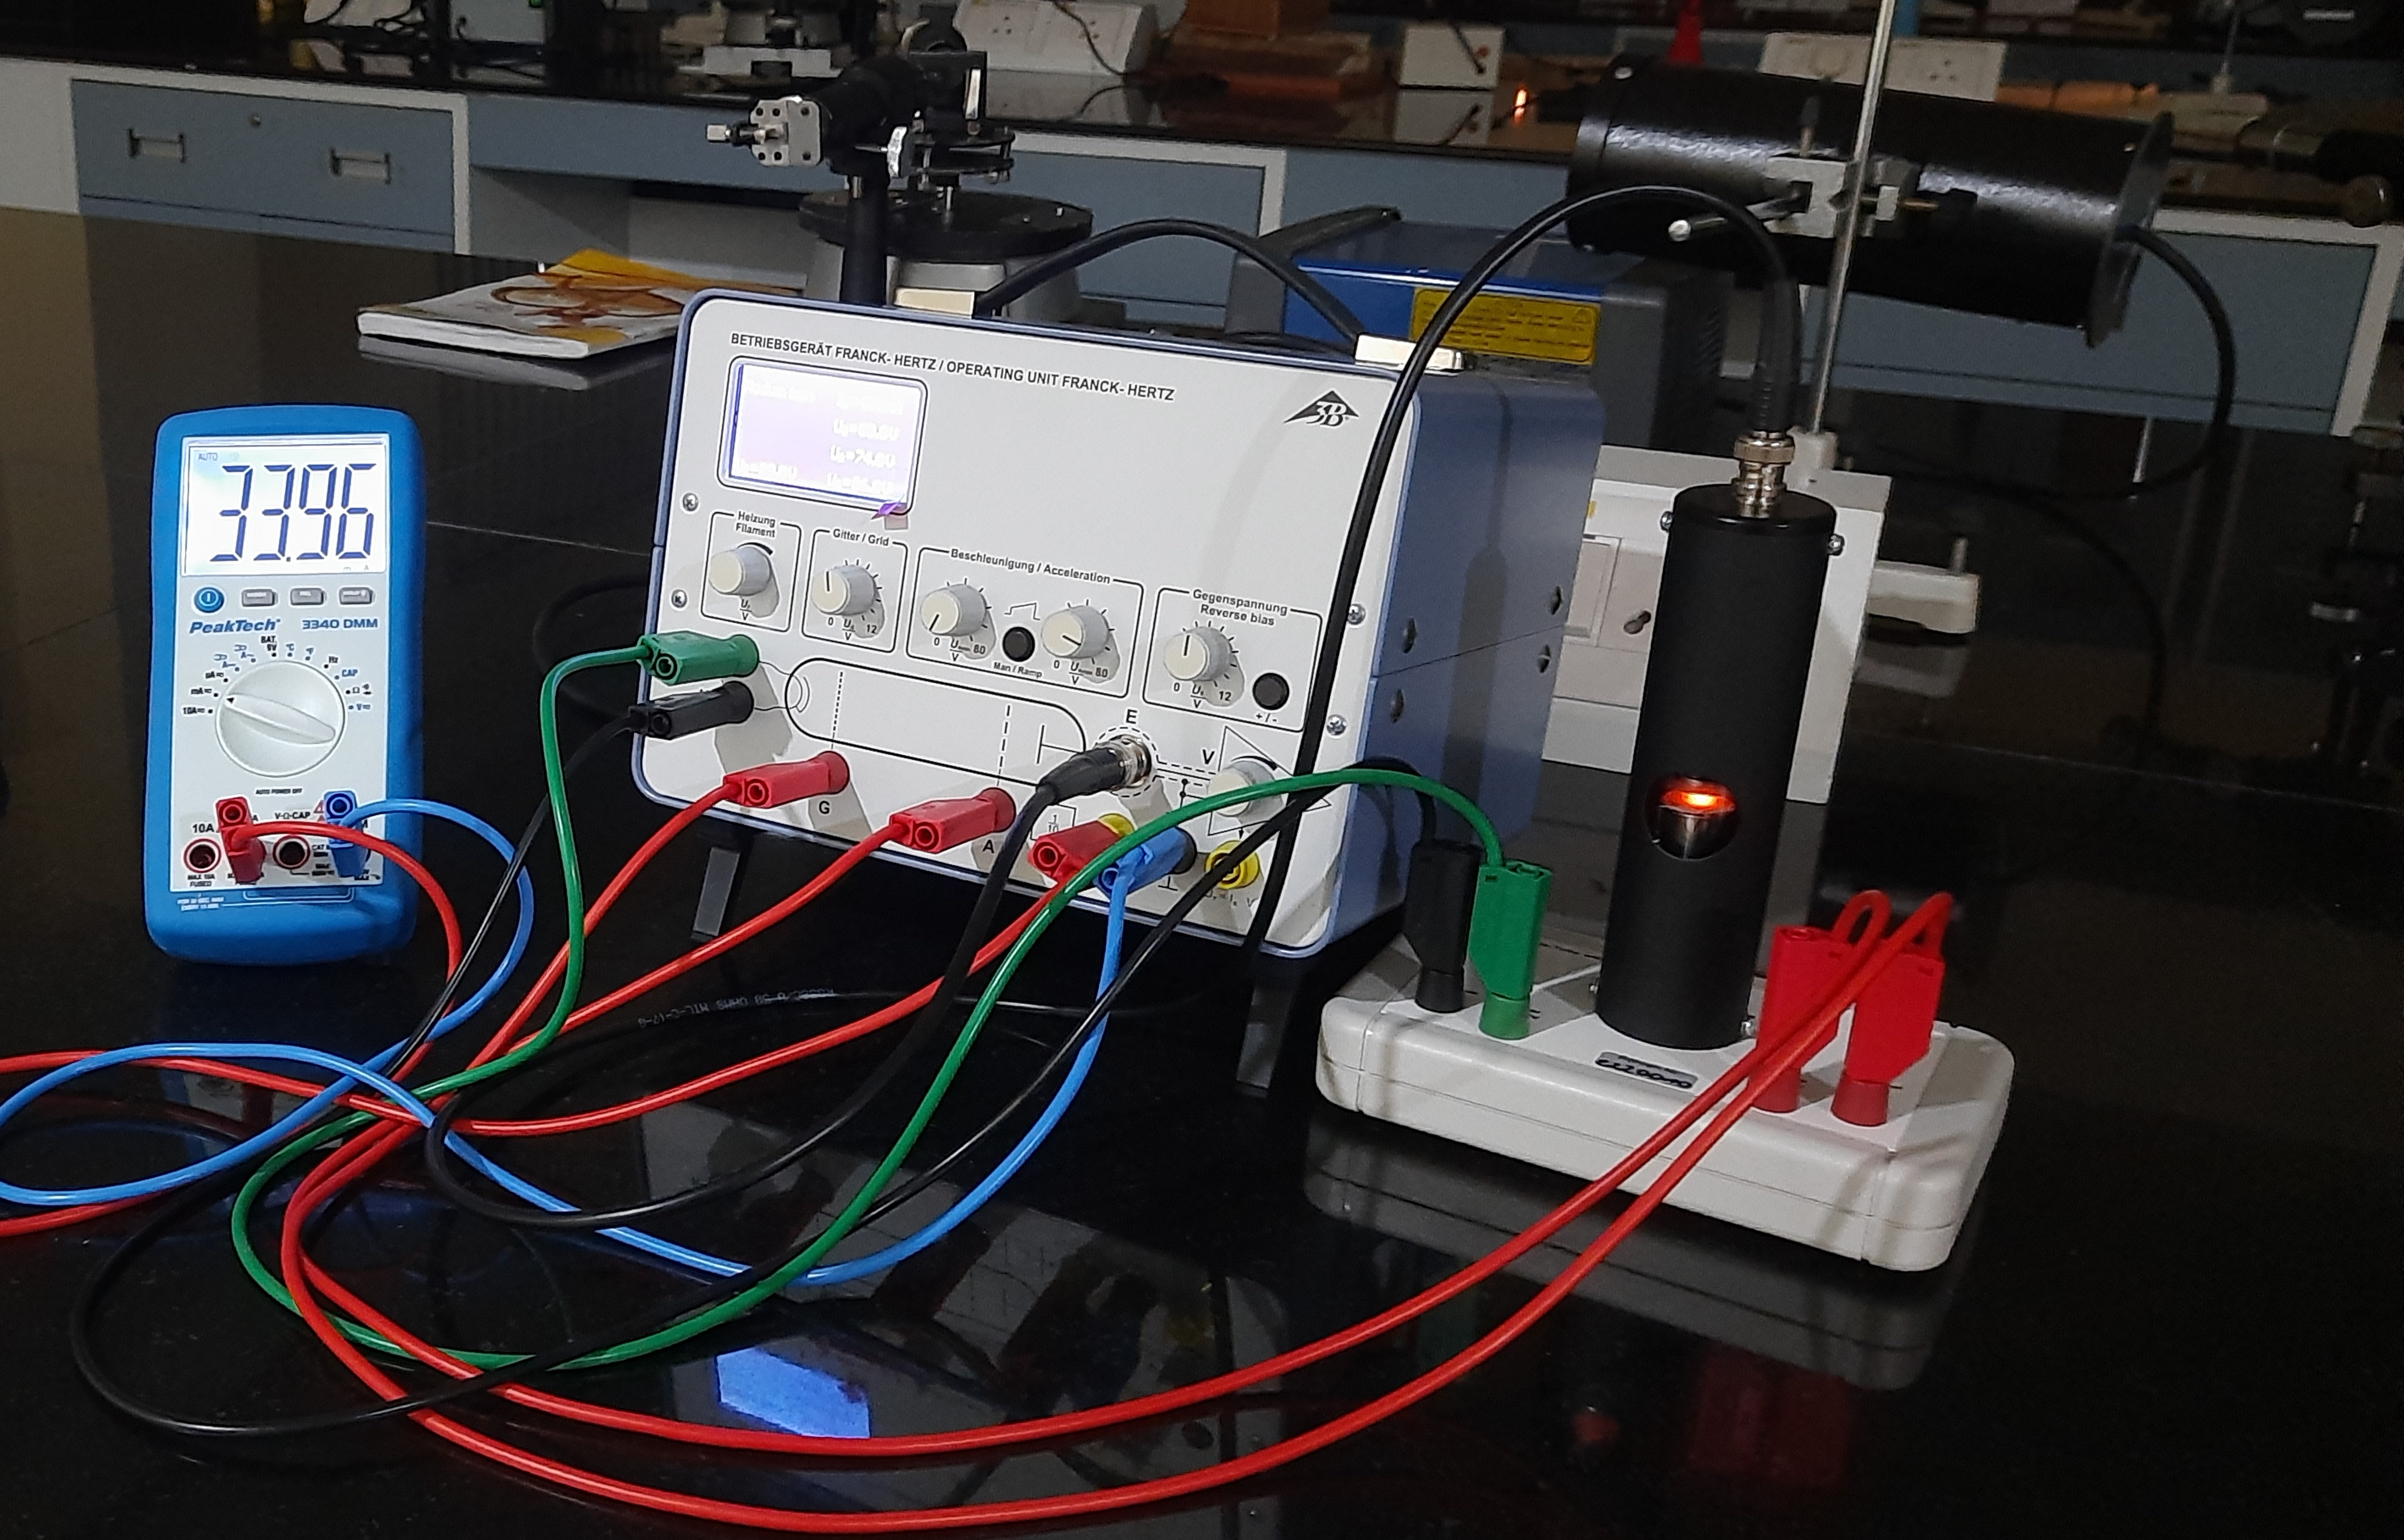
\includegraphics[width=8cm]{exp} 
   \caption{Experimental setup at laboratory}
   \label{ed}
\end{figure}

\subsection{Procedure}
The selector switch of the operating unit is set to manual mode and the tube is connected to the Franc-Hertz operating unit. Filament voltage is increased to around 8 V-9 V, it starts glowing. The breaking voltage is kept around 4 V - 8 V. The driving potential is kept around 4 V - 6 V. Keeping these voltages constant, vary the acceleration voltage and record the corresponding current. Repeat the experiment with different breaking, driving and filament voltage. Plot the graph between accelerating voltage versus collector current and determine the distance between two consecutive maxima to calculate the excitation energy. 

\subsection{Precautions}
\begin{enumerate}
\item{Turn the knobs carefully to note down the collector current.}
\item{Make sure the voltages applied do not exceed the mentioned limit.}
\item{Do not leave the apparatus over long duration as prolonged heating may reduce lifetime of cathode.}
\item{Start the experiment with the least value of knobs turned anticlockwise.}
\end{enumerate}

\section{Observation and Analysis}
\begin{figure}[H] %  figure placement: here, top, bottom, or page
   \centering
   \includegraphics[width=8cm]{i} 
   \caption{Luminescence visible layers in Neon tube.}
   \label{i}
\end{figure}

\begin{figure}[htbp] %  figure placement: here, top, bottom, or page
   \centering
   \includegraphics[width=9cm]{t1} 
   \caption{Plot of accelerating voltage versus collector current for table 1}
   \label{t1}
\end{figure}

It was observed that one could see the three layers of the glow due to excitation and de-excitation of the Neon atoms as mentioned in section (\ref{theo}). The plot of accelerating voltage versus collector current is shown in below figure. It is observed from the plot that maxima and minima at certain specific range is obtained. The average accelerating voltage is about 19.25 V, 18 V, 21 V and 19.5 V for Figure (5), Figure (6), Figure (7) and Figure (8), respectively. This is calculated by considering the distance between two maxima.  From the above obtained results, the average accelerating voltage is 19.438 V. Hence, accelerating voltage multiplied with electron charge gives the excitation energy of Neon atom. Therefore, the first excitation energy of Ne is 19.438 eV which is very close to the range 18.4-19 eV.  Sometimes due to double and multiple collisions of electrons and combinations of excitation of 3S level and 3P level, there may be small variations in plate current measured in nano-ampere. We also observe the three luminescence visible layers in Neon tube as shown in Figure (4).


The deviation in the experimentally obtained value could be due to random errors, human errors etc... Instrumental error also contribute to such deviations. It is difficult to perform the error analysis as the data was collected directly from the Franc-Hertz operating unit. It should also be noted that the data collection should be done quickly in order to avoid heating of the filament.

\begin{figure}[H] %  figure placement: here, top, bottom, or page
   \centering
   \includegraphics[width=9cm]{t2} 
   \caption{Plot of accelerating voltage versus collector current for table 2}
   \label{t2}
\end{figure}

\begin{figure}[H] %  figure placement: here, top, bottom, or page
   \centering
   \includegraphics[width=9.3cm]{t3} 
   \caption{Plot of accelerating voltage versus collector current for table 3}
   \label{t3}
\end{figure}

\begin{figure}[H] %  figure placement: here, top, bottom, or page
   \centering
   \includegraphics[width=9cm]{t4} 
   \caption{Plot of accelerating voltage versus collector current for table 4}
   \label{t4}
\end{figure}

\section{Conclusion}
The excitation energy of Ne atom was calculated as 19.438 eV by accelerating the electrons by thoriated activated cathode by thermionic emission, where inelastic collision takes place with the Ne atoms inside the Franc-Hertz tube. The electrons in the atom absorb the energy and get excited to higher energy state. The most probable excitation for Neon atoms takes place from ground states to ten 3p states, which is 18.4 eV and 19.0 eV from the ground state. The experimentally obtained value is close to this range. It was expected that the instrumental error contribute to this value as the readings were taken solely from operating unit.

\section{References}
\begin{enumerate}
\item{\url{https://www.niser.ac.in/sps/sites/default/files/basic_page/Franck-Hertz%20experiment_NISER.pdf}}
\item{\url{https://physicsx.erau.edu/Courses/CoursesS2022/PS315/Franck%20Hertz/experiment%20description.pdf}}
\item{\url{http://hyperphysics.phy-astr.gsu.edu/hbase/FrHz.html}}
\item{\url{https://en.wikipedia.org/wiki/Hot_cathode}}


\end{enumerate}

\end{document}